\chapter{Parecer Técnico} \label{cha:parecertecnico}

%%% Intro IA 
A inteligência sempre foi a característica mais notável do ser humano. Desde os primórdios, buscamos compreender como o nosso cérebro é capaz de perceber, aprender, raciocinar e agir em um mundo complexo e repleto de estímulos. Essa curiosidade levou cientistas e filósofos a tentarem reproduzir artificialmente aspectos do pensamento humano, primeiro em teorias e depois em máquinas capazes de simular comportamentos inteligentes. Com o avanço da computação e da matemática essas ideias deram origem ao campo da Inteligência Artificial (IA). A partir da década de 1950, nomes como Alan Turing e John McCarthy lançaram as bases teóricas e práticas da área, propondo as primeiras definições e experimentos em máquinas inteligentes \cite{haenlein2019brief}.

Segundo \textcite{russell2022}, o campo da IA ainda vai além de somente compreender a inteligência, mas também busca construir entidades inteligentes, capazes de realizar tarefas que normalmente exigem discernimento humano.
Gradualmente a IA evoluiu de sistemas baseados em regras fixas, nos quais as decisões eram determinadas por conjuntos explícitos de instruções programadas, para abordagens mais complexas de aprendizado de máquina (\textit{Machine Learning} - ML), e aprendizado profundo (\textit{Deep Learning} - DL). Essa evolução possibilitou o avanço de aplicações em diversas áreas distintas como saúde, indústria, entretenimento e comunicação \cite{nilsson2010quest}.

%%% Subareas IA
Cada subárea da IA se dedica a um tipo específico de desafio relacionado à reprodução da inteligência humana. Entre as principais, destacam-se o ML, que permite aos sistemas identificar padrões e melhorar seu desempenho a partir de dados; o DL, baseado em redes neurais com múltiplas camadas, capaz de reconhecer imagens, sons e textos; e a visão computacional, responsável por interpretar e compreender imagens e vídeos.
Outras subáreas relevantes incluem o reconhecimento de fala, que converte áudio em texto e dá suporte a assistentes virtuais; sistemas especialistas, projetados para apoiar a tomada de decisão em domínios específicos; o planejamento automatizado, que define sequências de ações para atingir objetivos; e a robótica inteligente, que combina percepção através de sensores, planejamento e ação em ambientes físicos.
Também há o Processamento de Linguagem Natural (\textit{Natural Language Processing} - NLP), foco do presente parecer técnico, que se destaca como o campo voltado a ensinar máquinas a compreender e produzir linguagem humana \cite{russell2022}.

%%% NLP IA
A subárea da NLP se destaca por tentar ensinar máquinas a compreender, interpretar e produzir linguagem humana. Essa tarefa é desafiadora, pois a linguagem é ambígua, contextual e profundamente dependente de contexto cultural e situacional. Computadores lidam facilmente com linguagens estruturadas, como as de programação, mas têm dificuldade em compreender a linguagem natural, que depende de significados e intenções humanas.

%%% Exemplo NLP 
Por exemplo, note como um computador pode compreender e executar com precisão um código em Python, no qual as condições e ações estão claramente definidas, conforme o Algoritmo~\ref{alg:dumbledore}.
\begin{algorithm}[H]
\centering
\caption{Instrução literal em código Python}
\vspace{0.5em}
\begin{lstlisting}[language=Python, style=input]
# Código que o computador entende
dumbledore_tem_telescopio = True
homem_tem_telescopio = False

if dumbledore_tem_telescopio:
    print("Dumbledore usou o telescópio para observar o homem.")
elif homem_tem_telescopio:
    print("Dumbledore viu o homem que estava com o telescópio.")
else:
    print("Não há telescópio envolvido na observação.")
\end{lstlisting}
\caption*{Fonte: O autor (2025).}
\label{alg:dumbledore}
\end{algorithm}
\vspace{-0.5em}
Já uma instrução equivalente em linguagem natural, no caso em português, conforme o Quadro~\ref{quadroo:ambiguidade}.
\begin{quadroo}[H]
\centering
\caption{Instrução ambígua em linguagem natural}
\vspace{0.5em}
\begin{tcolorbox}[
  colback=yellow!20, 
  colframe=black,
  width=0.8\linewidth,   % largura do box igual ao lstlisting
  left=0pt,               % remove deslocamento interno
  boxsep=2mm,
  enlarge left by=-0.02\linewidth  % desloca o box inteiro para direita
]
Se Dumbledore viu o homem com o telescópio, mostre uma mensagem adequada descrevendo a situação.
\end{tcolorbox}
\caption*{Fonte: O autor (2025).}
\label{quadroo:ambiguidade}
\end{quadroo}
\vspace{-0.5em}
Nessa frase, não está claro quem possui o telescópio, Dumbledore ou o homem observado, pois a linguagem natural é ambígua e dependente de contexto. Essa ambiguidade é natural para os humanos, que usam o contexto para entender o sentido, mas é um desafio para os computadores.
Enquanto o código define explicitamente cada condição para que a máquina execute a ação correta, a linguagem humana exige interpretação e inferência, habilidades que os computadores não possuem de forma nativa.
O NLP surge exatamente para reduzir essa lacuna, permitindo que sistemas computacionais compreendam e produzam linguagem humana de maneira mais contextualizada e natural, ampliando a interação entre pessoas e máquinas.

%%% Linguistica NLP
Um dos maiores desafios do NLP é lidar com a ambiguidade linguística. A linguagem humana raramente tem um único significado literal, palavras e frases podem variar de sentido conforme o contexto. A ambiguidade mostra que compreender linguagem natural exige mais do que reconhecer palavras, é preciso entender estrutura sintática, significado semântico e contexto pragmático \cite{jurafsky2023speech}.

Assim, o NLP não é apenas um processamento de texto, mas uma tentativa de modelar matematicamente a própria complexidade da linguagem. Essa aproximação entre linguística e computação não é recente: desde a década de 1950, linguistas como Noam Chomsky discutem estruturas formais da linguagem que inspiraram modelos computacionais de análise sintática e semântica \cite{chomsky1957syntactic}.

%%% Tradução idiomas NLP
Uma das aplicações mais antigas do NLP é a tradução entre línguas, cuja evolução demonstra claramente a importância do contexto linguístico. Conforme \textcite{hutchins2005history}, os primeiros tradutores criados usavam regras gramaticais rígidas, gerando traduções literais e muitas vezes incorretas.
Com o avanço dos métodos estatísticos e das redes neurais, as traduções passaram a considerar o contexto e os padrões linguísticos aprendidos em grandes volumes de dados.
Em vez de traduzir palavra por palavra, os sistemas modernos, como o \textit{Google Translate} e o \textit{DeepL}, analisam frases completas e o sentido geral, levando em conta o significado geral e a probabilidade de combinações linguísticas, produzindo traduções mais naturais e próximas da linguagem humana.

%%% LLMS NLP
Outra aplicação da NLP popularmente conhecida ultimamente são os chamados Modelos de Linguagem de Grande Escala (\textit{Large Language Models} - LLMs), como o \textit{ChatGPT}. Tais modelos são capazes de compreender e gerar texto de forma coerente, criando respostas contextualizadas, resumos, traduções e até textos criativos. O funcionamento das LLMs baseia-se em arquiteturas de redes DL, especialmente na arquitetura  \textit{transformer}, introduzida por \textcite{vaswani2017attention}, que permite analisar várias palavras ao mesmo tempo e entender relações de longo alcance dentro de um texto.

Os impactos das LLMs vão além da tecnologia, eles transformaram a forma como interagimos com a tecnologia, permitindo a comunicação natural entre humanos e máquinas. Sistemas baseados em NLP são empregados em assistentes virtuais, ferramentas de revisão gramatical, análise de sentimentos, geração de conteúdo e ensino de idiomas, demonstrando o potencial da IA em compreender e reproduzir aspectos cada vez mais complexos da linguagem. Nos últimos anos, o avanço de modelos de linguagem em larga escala transformou a pesquisa em NLP e linguística computacional, aproximando máquinas da capacidade humana de gerar e compreender texto natural \cite{bommasani2021opportunities}.


\begin{figure}[h!]
\centering
\caption{Inter-relações entre os subcampos da Inteligência Artificial e Linguística}
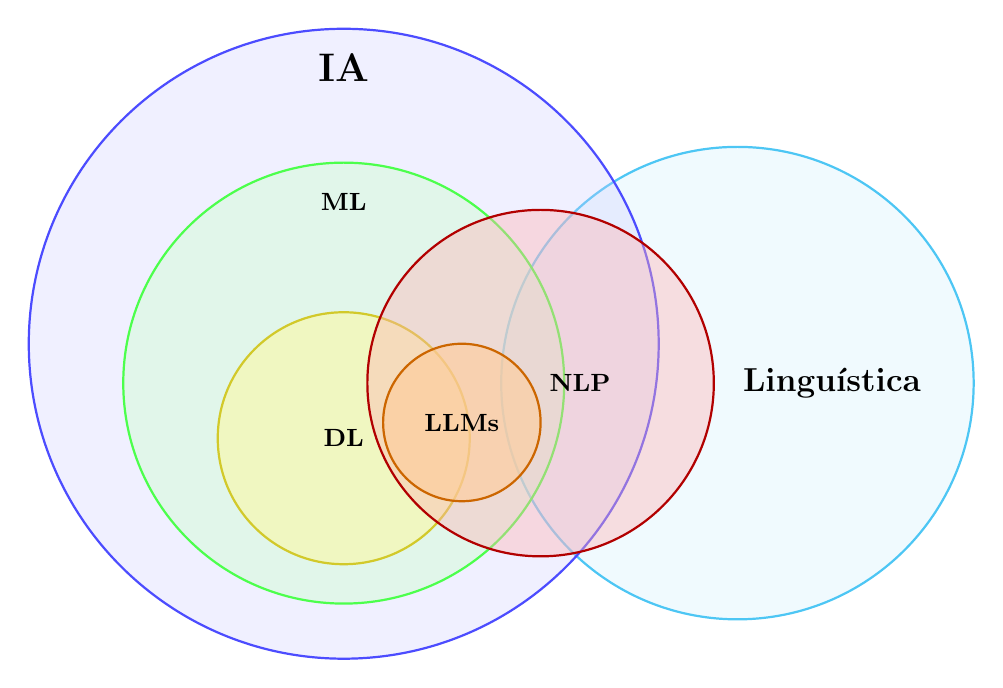
\begin{tikzpicture}[scale=1.0, every node/.style={align=center, font=\small}]

% --- Linguística ---
\filldraw[fill=cyan!20, fill opacity=0.3, draw=cyan!70, thick] (5,-0.5) circle (3cm);
\node at (6.2,-0.5) {\large \textbf{Linguística}};

% --- Inteligência Artificial ---
\filldraw[fill=blue!20, fill opacity=0.3, draw=blue!70, thick] (0,0) circle (4cm);
\node at (0,3.5) {\Large \textbf{IA}};

% --- Machine Learning ---
\filldraw[fill=green!20, fill opacity=0.4, draw=green!70, thick] (0,-0.5) circle (2.8cm);
\node at (0,1.8) {\textbf{ML}};

% --- Deep Learning ---
\filldraw[fill=yellow!40, fill opacity=0.5, draw=yellow!80!black, thick] (0,-1.2) circle (1.6cm);
\node at (0,-1.2) {\textbf{DL}};

% --- NLP ---
\filldraw[fill=red!30, fill opacity=0.4, draw=red!70!black, thick] (2.5,-0.5) circle (2.2cm);
\node at (3.0,-0.5) {\textbf{NLP}};

% --- LLM ---
\filldraw[fill=orange!40, fill opacity=0.6, draw=orange!80!black, thick] (1.5,-1.0) circle (1.0cm);
\node at (1.5,-1.0) {\textbf{LLMs}};

\end{tikzpicture}\caption*{Fonte: O autor (2025).}
\label{fig:vennIA}
\end{figure}

%%
A Figura~\ref{fig:vennIA} ilustra, de forma conceitual, a relação entre os principais campos da IA aplicados a NLP e suas interconexões com a Linguística. Vale destacar que, se o foco do presente parecer fosse outra subárea da IA, como visão computacional ou robótica, a figura apresentaria uma estrutura diferente, refletindo outras intersecções entre diferentes domínios de estudo.

O diagrama foi concebido com base nas referências estudadas sobre os temas apresentados, aliadas às interpretações pessoais desenvolvidas ao longo do curso. A construção do diagrama foi realizada utilizando o pacote \texttt{TikZ} do ambiente \LaTeX{}, e a escolha de círculos sobrepostos reflete a natureza interdependente e contínua das fronteiras entre esses campos.

A IA constitui o campo mais abrangente, englobando diversas abordagens voltadas à construção de sistemas inteligentes. Dentro dela, o ML representa uma subárea que permite às máquinas aprenderem a partir de dados, enquanto o DL surge como uma vertente mais específica, baseada em redes neurais com múltiplas camadas. 
O NLP aparece como uma área de interseção entre a IA e a Linguística, pois combina técnicas computacionais e conhecimento linguístico para interpretar e gerar linguagem humana. 

Por fim, as LLMs representam um avanço recente e significativo dentro desse contexto, pois aplicam algoritmos de aprendizado profundo em larga escala para compreender e produzir texto com alto grau de coerência. Dessa forma, a figura sintetiza como essas áreas e subáreas se sobrepõem e se complementam, refletindo a natureza interdisciplinar e dinâmica da inteligência artificial moderna.